% =============================================================================
% DASF-Net: Dual-Adversarial Spectral Fusion for Cross-Lingual and
% Adversarially Robust Audio Deepfake Detection
%
% IEEE conference-format LaTeX source.
% Build: pdflatex -> pdflatex (bibliography is inline, no bibtex pass needed)
%
% SCOPE OF THIS DRAFT: architecture, methodology, algorithms and experimental
% design only. The Results section is deliberately ABSENT and must be written
% after the experiments of Section VII are run.
% =============================================================================
\documentclass[conference]{IEEEtran}
\IEEEoverridecommandlockouts

\usepackage{cite}
\usepackage{amsmath,amssymb,amsfonts}
\usepackage{algorithm}
\usepackage{algorithmic}
\usepackage{graphicx}
\usepackage{textcomp}
\usepackage{xcolor}
\usepackage{booktabs}
\usepackage{multirow}
\usepackage{url}
\usepackage[hidelinks]{hyperref}

% Float placement: three full-width figures plus two algorithms compete for
% top slots; without these the figure* floats are deferred past the
% bibliography.
\setcounter{topnumber}{2}
\setcounter{bottomnumber}{2}
\setcounter{totalnumber}{4}
\renewcommand{\topfraction}{0.92}
\renewcommand{\bottomfraction}{0.7}
\renewcommand{\textfraction}{0.06}
\renewcommand{\floatpagefraction}{0.65}

\newcommand{\Loss}{\mathcal{L}}
\newcommand{\Dsrc}{\mathcal{D}_{\mathrm{src}}}
\newcommand{\Dtgt}{\mathcal{D}^{u}_{\mathrm{tgt}}}

\def\BibTeX{{\rm B\kern-.05em{\sc i\kern-.025em b}\kern-.08em
    T\kern-.1667em\lower.7ex\hbox{E}\kern-.125emX}}

% -----------------------------------------------------------------------------
% REFERENCES SUPPRESSED IN THIS DRAFT.
% \cite is redefined to print nothing (\unskip swallows the space that would
% otherwise be left behind), and the thebibliography block at the end of the
% file is wrapped in \iffalse ... \fi.
%
% TO RESTORE REFERENCES: delete the \renewcommand line below, and delete the
% \iffalse / \fi lines surrounding the bibliography at the end of this file.
% Every \cite key is still in place, so nothing else needs editing.
% -----------------------------------------------------------------------------
\renewcommand{\cite}[1]{\unskip}

\begin{document}

\title{DASF-Net: Dual-Adversarial Spectral Fusion for\\
Cross-Lingual and Adversarially Robust Audio Deepfake Detection}

% All three authors share one affiliation, so a single centred block is used;
% three side-by-side \IEEEauthorblockN columns overflow the text width and
% wrap the third author onto its own left-aligned line.
\author{
\IEEEauthorblockN{Iftikhar Ahmed,\quad Meherun Nessa Mithila,\quad Mohammad Abdul Qayum}
\IEEEauthorblockA{\textit{Department of Electrical and Computer Engineering}\\
\textit{North South University}, Dhaka, Bangladesh\\
\{iftikhar.ahmed,\ meherun.mithila,\ mohammad.qayum\}@northsouth.edu}
}

\maketitle

\begin{abstract}
Audio deepfake detectors are trained and evaluated almost exclusively on
high-resource languages and on a narrow family of neural vocoders. When such
a detector meets a new language synthesised by a structurally different
generator, two failure modes compound: the learned features encode
language- and corpus-specific cues rather than synthesis artifacts, and the
decision boundary remains trivially breakable by gradient-based
perturbation. We propose \textbf{DASF-Net}, a detection architecture built
around the observation that these two failures are both \emph{adversarial}
problems and can be attacked with a single training formulation. DASF-Net
couples (i) a dual-branch spectral front-end that presents the same
utterance as a sparse cepstral view (LFCC) and a dense spectral view
(log-Mel) to one Siamese-shared, ImageNet-pretrained Xception trunk; (ii) a
\emph{Cross-Attention Spectral Fusion} (CASF) module that lets the two views
query one another and combines them through a learned gate, so the network
selects per utterance which representation carries the artifact; and (iii) a
\emph{dual-adversarial} objective in which a gradient-reversed language
discriminator drives the embedding toward language invariance while
adaptive FGSM/PGD adversarial training drives it toward perturbation
robustness. A three-stage curriculum trains the parts in a stable order. We
instantiate the design on the English WaveFake corpus (117,985 utterances,
seven GAN- and flow-based vocoders) as source domain and the Bengali
BanglaFake corpus (25,520 utterances, one VITS end-to-end system) as target
domain, a pairing that varies language and synthesis paradigm at once. We
further specify a Confound-Controlled Evaluation Protocol that neutralises
the speaker, gender and class-prior imbalances which otherwise inflate
Bengali detection scores. This paper presents the architecture, the training
algorithms and the experimental design; the empirical study is reported
separately.
\end{abstract}

\begin{IEEEkeywords}
audio deepfake detection, cross-lingual generalisation, adversarial
robustness, domain-adversarial training, cross-attention fusion,
Mel-spectrogram, Xception, Bengali speech, low-resource language
\end{IEEEkeywords}

% =============================================================================
\section{Introduction}
% =============================================================================

Neural vocoders and end-to-end text-to-speech (TTS) systems now produce
speech that listeners routinely fail to separate from genuine recordings
\cite{kong2020hifigan,kumar2019melgan,prenger2019waveglow,yamamoto2020pwg,kim2021vits}.
The resulting misuse --- voice-impersonation fraud, fabricated evidence,
political disinformation --- has driven a decade of work on automatic
detection \cite{todisco2019asvspoof,frank2021wavefake}. That work is
overwhelmingly English, and overwhelmingly built on a single family of
generators. Bengali, with more than 230 million native speakers, has almost
no detection literature: BanglaFake \cite{fahad2025banglafake} first made
Bengali deepfake audio available at scale but trained no detector, and
``Zero-Shot to Zero-Lies'' \cite{samu2025zeroshot} first benchmarked
detectors on it, reporting a best zero-shot result of 53.80\% accuracy
(46.20\% EER, Wav2Vec2-XLSR-53) and a best fine-tuned result of 79.17\%
accuracy (24.35\% EER, ResNet18).

Those numbers expose a gap that is not merely quantitative. A detector that
transfers this poorly is not simply under-trained; it has learned the wrong
thing. Its features encode which corpus, which speaker and which language
produced an utterance, rather than what a synthesiser did to it. The same
detector is also, as a large body of adversarial work shows, breakable by
perturbations far below the audible threshold: Kawa \emph{et al.}
\cite{kawa2023lcnn} degrade an LCNN countermeasure from 0.022 to 0.785 EER
under FGSM, and our own prior study \cite{ahmed2026melspec} reproduces the
pattern on a much larger ImageNet-pretrained Xception detector.

\subsection{From measuring a gap to closing it}
Prior cross-lingual studies characterise the degradation and stop there.
Our position is that the two failures above share a structure. In both
cases the network has latched onto a nuisance direction in feature space
--- language and corpus identity in one case, a locally exploitable
gradient direction in the other --- and in both cases the standard remedy
is to introduce an adversary that penalises exactly that direction.
Domain-adversarial training \cite{ganin2016dann} supplies the first adversary;
FGSM/PGD adversarial training \cite{goodfellow2015fgsm,madry2018pgd}
supplies the second. Placing both on a single shared embedding is, to our
knowledge, new for audio deepfake detection, and it turns the cross-lingual
question from a measurement exercise into an architectural one.

A second, independent question concerns \emph{which} spectral
representation a convolutional detector should consume. Linear Frequency
Cepstral Coefficients (LFCC) have been the default for spoofing
countermeasures since the Gaussian-Mixture-Model era \cite{frank2021wavefake},
yet our prior study showed that for CNNs the ordering reverses:
dense 128-bin log-Mel spectrograms outperform 20-coefficient LFCC by a
consistent 33--35\% relative EER margin across all seven WaveFake vocoders,
because dense two-dimensional inputs suit both convolutional inductive bias
and ImageNet transfer. That study treated the two representations as
mutually exclusive alternatives and explicitly left hybrid representations
as future work. DASF-Net takes up that thread: rather than choosing, it
consumes both and learns a per-utterance gate between them.

\subsection{Contributions}
\begin{enumerate}
\item \textbf{DASF-Net}, an architecture that presents sparse cepstral and
dense spectral views of one utterance to a single Siamese-shared Xception
trunk and fuses them with a two-way cross-attention module and a learned
gate (Section~\ref{sec:arch}).
\item A \textbf{dual-adversarial objective} that combines a
gradient-reversed language discriminator with adaptive FGSM/PGD adversarial
training on the same fused embedding, together with a three-stage
curriculum that makes the combination trainable (Section~\ref{sec:training}).
\item A \textbf{Confound-Controlled Evaluation Protocol} (CCEP) for
Bengali--English deepfake transfer, which neutralises the speaker, gender
and class-prior artifacts that make naive BanglaFake accuracy figures
uninterpretable, and a corrected, unit-consistent adversarial threat model
(Sections~\ref{sec:threat} and \ref{sec:design}).
\item An experimental design that separates the contribution of each
component through ablation, so that any cross-lingual gain can be
attributed rather than merely observed (Section~\ref{sec:design}).
\end{enumerate}

This paper is deliberately scoped to design and methodology. No empirical
results are reported here.

\begin{figure*}[!t]
\centering
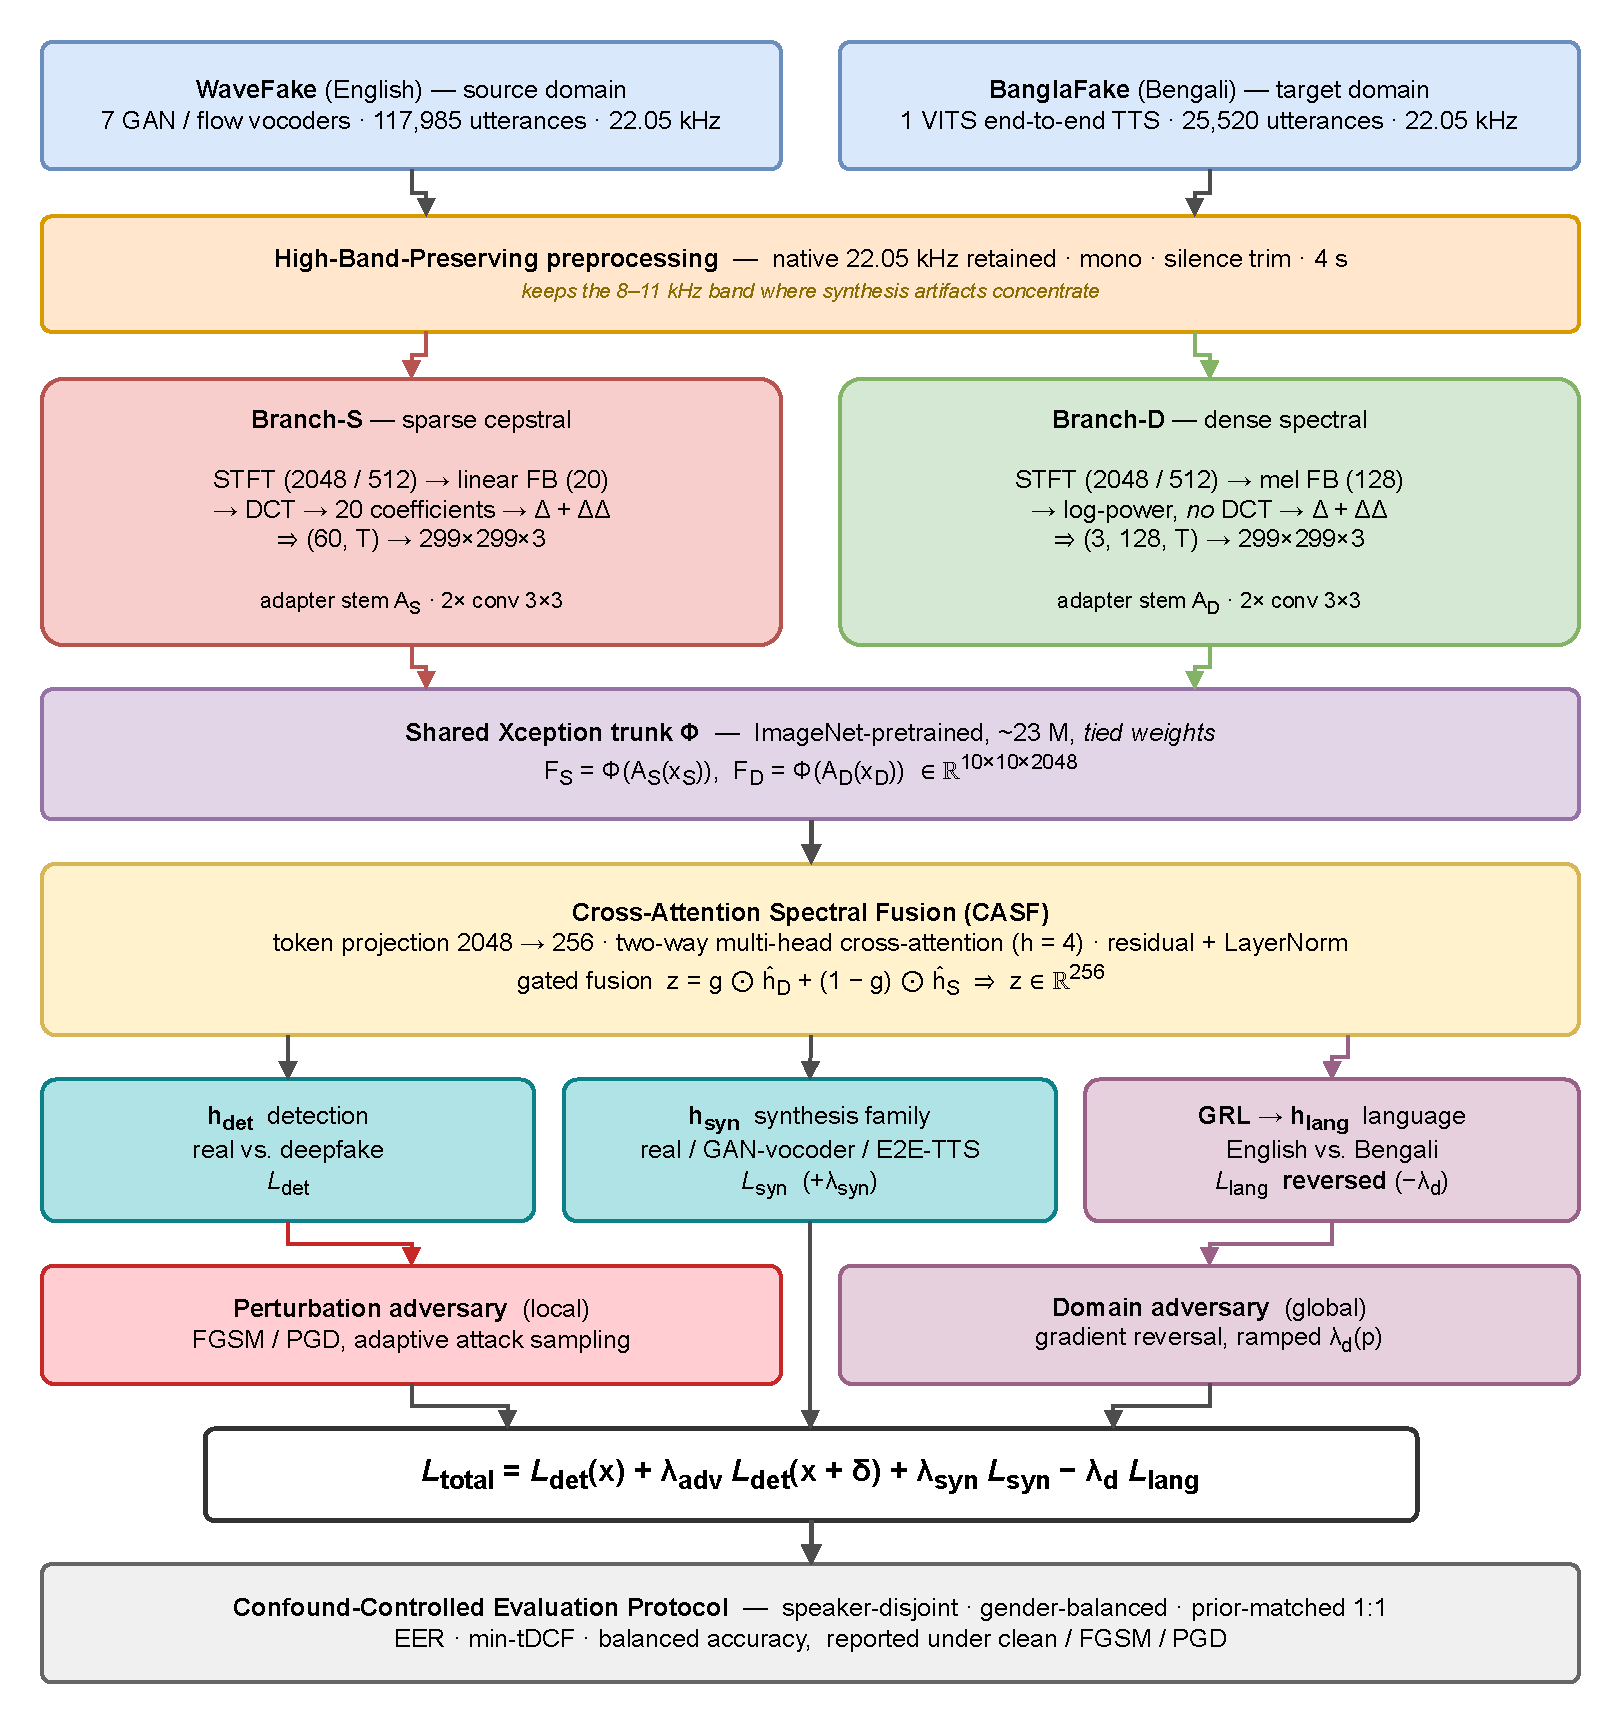
\includegraphics[width=0.94\textwidth]{fig1-methodology.drawio.pdf}
\caption{End-to-end DASF-Net methodology. Both corpora pass through
identical High-Band-Preserving preprocessing, split into a sparse cepstral
and a dense spectral branch, and are encoded by one Siamese-shared Xception
trunk. Cross-Attention Spectral Fusion produces a single embedding $z$ on
which three heads act: detection, an auxiliary synthesis-family classifier,
and a gradient-reversed language discriminator. Two adversaries ---
perturbation and domain --- shape the same embedding through the combined
objective, and all reported figures follow the Confound-Controlled
Evaluation Protocol.}
\label{fig:pipeline}
\end{figure*}

% =============================================================================
\section{Related Work}
% =============================================================================

\subsection{Datasets and benchmarks}
ASVspoof \cite{todisco2019asvspoof} and the ADD challenge series
standardised English and Chinese anti-spoofing evaluation. WaveFake
\cite{frank2021wavefake} contributed 117,985 utterances spanning seven
neural vocoders derived from LJSpeech \cite{ito2017ljspeech}, enabling
leave-one-vocoder-out study of cross-generator generalisation. BanglaFake
\cite{fahad2025banglafake} pairs 12,260 real Bengali utterances (SUST TTS
Corpus \cite{ahmad2021sust}, Mozilla Common Voice \cite{ardila2020commonvoice})
with 13,260 utterances from a VITS \cite{kim2021vits} system trained on the
SUST corpus; its authors assess dataset quality by Mean Opinion Score and a
t-SNE view of MFCC features, reporting substantial overlap between the real
and synthetic clusters, but train no detector. The Zero-Shot to Zero-Lies benchmark
supplied the first Bengali detection benchmark over zero-shot pretrained
models (Wav2Vec2-XLSR-53, Whisper, PANNs-CNN14, WavLM, AST) and fine-tuned
architectures (Wav2Vec2-Base, LCNN, LCNN-Attention, ResNet18, ViT-B/16,
CNN-BiLSTM).

\subsection{Feature representations for CNN detectors}
LFCC with a GMM back-end long dominated countermeasure design, and the
WaveFake study adopted it as its baseline. Our prior work showed the advantage is
back-end-specific: a dense 128-bin log-Mel spectrogram transfers far better
into an ImageNet-pretrained Xception CNN \cite{chollet2017xception} than a
sparse 20-coefficient cepstral representation, because the former retains
the two-dimensional time--frequency structure that convolution and
ImageNet initialisation both assume. Whether that advantage is specific to
GAN-vocoder artifacts, or survives a change of synthesis paradigm and
language, motivates the present architecture. Multi-view and multi-branch
front-ends are established elsewhere in speech, but we are not aware of a
learned, attention-gated fusion of cepstral and spectral views for deepfake
detection.

\subsection{Domain-adversarial and cross-lingual transfer}
Domain-adversarial neural networks \cite{ganin2016dann} attach a domain
classifier through a gradient reversal layer so that the shared encoder is
trained to be uninformative about domain while remaining discriminative for
the task. The technique is standard in vision and in speech recognition,
but it has not, to our knowledge, been applied to make an audio deepfake
detector language-invariant. Both the BanglaFake dataset paper and
the Zero-Shot to Zero-Lies benchmark name cross-lingual generalisation as open for
Bengali; neither proposes a mechanism for it.

\subsection{Adversarial robustness of countermeasures}
FGSM \cite{goodfellow2015fgsm} and PGD \cite{madry2018pgd} are the standard
white-box stress tests. Kawa et al. demonstrated catastrophic LCNN
degradation under FGSM and partial recovery through adversarial training at
a clean-accuracy cost. Our prior study reproduced this on Xception
with an adaptive scheme that samples attacks in proportion to a
momentum-smoothed estimate of their recent success. No prior work examines
adversarial robustness for Bengali deepfake detection, nor whether
robustness acquired in one language survives transfer to another.

% =============================================================================
\section{Datasets}
% =============================================================================

\subsection{WaveFake (English, source domain)}
WaveFake \cite{frank2021wavefake} contains 117,985 utterances (13,100 real,
104,885 synthetic) built from the single-speaker LJSpeech corpus
\cite{ito2017ljspeech}: MelGAN, MelGAN-Large, Parallel WaveGAN,
Multi-Band MelGAN, Full-Band MelGAN, HiFi-GAN and WaveGlow, plus a full TTS
pipeline. All are GAN-based or GAN-adjacent flow vocoders that
\emph{resynthesise} a waveform from acoustic features of real speech.

\subsection{BanglaFake (Bengali, target domain)}
BanglaFake \cite{fahad2025banglafake} contains 25,520 utterances: 12,260
real (10,000 SUST TTS Corpus, 2,260 Common Voice across five speakers) and
13,260 synthesised by a single VITS model trained from scratch on the SUST
corpus. VITS is an end-to-end variational/flow architecture that generates
speech from text without an intermediate acoustic-feature stage, and is
therefore structurally unlike every WaveFake generator. Audio is
distributed as 22{,}050~Hz WAV, 6--7~s per clip, in LJSpeech-style layout.

\subsection{Why this pairing, and what it confounds}
\label{sec:pairing}
Because language and synthesis paradigm change together, English
$\leftrightarrow$ Bengali transfer probes cross-lingual \emph{and}
cross-architecture generalisation simultaneously. That is the property we
want, but the pairing also carries three confounds that any honest
evaluation must neutralise, and that we address in
Section~\ref{sec:design}:

\begin{enumerate}
\item \textbf{Speaker and gender.} BanglaFake's synthetic side is one male
speaker while its real side spans seven speakers of both genders. A
detector can score highly by classifying gender rather than artifacts.
\item \textbf{Class prior.} WaveFake is roughly 8:1 synthetic-to-real;
BanglaFake is roughly 1:1. Accuracy is not comparable across such
different priors, and a threshold calibrated on one is miscalibrated on the
other.
\item \textbf{Bandwidth.} Both corpora are natively 22.05~kHz. Downsampling
to 16~kHz, as in our prior study and much prior work, discards
everything above 8~kHz --- precisely the band in which vocoder and
end-to-end TTS artifacts are most pronounced, and the band most likely to
differ between the two generator families.
\end{enumerate}

Table~\ref{tab:datasets} summarises both corpora after the alignment of
Section~\ref{sec:hbp}.

\begin{table}[htbp]
\caption{Dataset summary after High-Band-Preserving alignment}
\label{tab:datasets}
\centering
\begin{tabular}{lcc}
\toprule
& \textbf{WaveFake} & \textbf{BanglaFake} \\
\midrule
Role & source & target \\
Language & English & Bengali \\
Real utterances & 13,100 & 12,260 \\
Synthetic utterances & 104,885 & 13,260 \\
Synthesis family & 7, GAN / flow & 1, VITS end-to-end \\
Speaker(s), synthetic & 1 female & 1 male \\
Speaker(s), real & 1 female & 7 (mixed gender) \\
Source corpus & LJSpeech & SUST TTS Corpus \\
Sample rate (retained) & 22,050~Hz & 22,050~Hz \\
\bottomrule
\end{tabular}
\end{table}

% =============================================================================
\section{Proposed Architecture: DASF-Net}
\label{sec:arch}
% =============================================================================

Figure~\ref{fig:pipeline} gives the whole method; Fig.~\ref{fig:dasfnet}
expands the network itself. We describe each component and the reason it is
present.

\subsection{High-Band-Preserving preprocessing}
\label{sec:hbp}
Every utterance from both corpora is brought to a common representation:
mono, native 22.05~kHz \emph{retained}, silences longer than 2~s trimmed at
a 40~dB threshold, and duration normalised to 4~s by centre-cropping or
reflection padding. Retaining the native rate is a deliberate departure
from \cite{ahmed2026melspec}. Downsampling to 16~kHz imposes an 8~kHz
Nyquist ceiling and removes the 8--11~kHz band; for a within-corpus study
that loss is tolerable, but for a cross-\emph{paradigm} claim it silently
deletes the evidence most likely to distinguish a GAN vocoder from an
end-to-end model. All filterbanks below therefore run to
$f_{\max} = 11.025$~kHz.

\subsection{Dual-branch spectral front-end}
Both branches share Short-Time Fourier Transform parameters
($n_{\mathrm{fft}} = 2048$, hop $= 512$), so any difference between them is
attributable to the filterbank and compression stages alone.

\textbf{Branch-S (sparse cepstral).} Linear-frequency filterbank
(20 filters, 0--11.025~kHz) $\rightarrow$ Discrete Cosine Transform
$\rightarrow$ 20 cepstral coefficients $\rightarrow$ first and second
temporal derivatives, giving a $(60, T)$ representation.

\textbf{Branch-D (dense spectral).} Mel-scaled filterbank
($n_{\mathrm{mels}} = 128$, $f_{\max} = 11.025$~kHz) $\rightarrow$
log-power compression, with \emph{no} DCT, so the dense time--frequency
structure survives $\rightarrow$ first and second derivatives, giving a
$(3, 128, T)$ tensor.

Both are resized to $299 \times 299 \times 3$, the Xception input geometry.
Branch-S preserves the sharp, high-frequency periodicities on a linear
scale that made LFCC effective for statistical back-ends; Branch-D
preserves the dense spatial structure that convolution exploits. The two
are complementary rather than competing, which is the premise of the fusion
module.

\subsection{Branch adapters and a Siamese-shared trunk}
Each branch owns a small \emph{adapter stem} $A_S$, $A_D$ --- two
$3\times3$ convolutions with batch normalisation and ReLU, about $0.06$~M
parameters each --- whose role is to map branch-specific input statistics
into a common range before the shared encoder sees them.

The encoder $\Phi$ is a single ImageNet-pretrained Xception
\cite{chollet2017xception} ($\approx 23$~M parameters) applied to both
branches with tied weights:
\begin{equation}
F_S = \Phi(A_S(x_S)), \qquad F_D = \Phi(A_D(x_D)),
\end{equation}
with $F_S, F_D \in \mathbb{R}^{10 \times 10 \times 2048}$. Weight sharing is
a design commitment, not an economy: two independent backbones would let
each branch build a private feature space, and the fusion module would then
have to reconcile two unrelated geometries. One trunk forces both views
into a single artifact space at the cost of $0.12$~M extra adapter
parameters, and keeps the model comparable in size to the single-branch
baseline of \cite{ahmed2026melspec}.

\subsection{Cross-Attention Spectral Fusion (CASF)}
\label{sec:casf}

\begin{figure*}[!t]
\centering
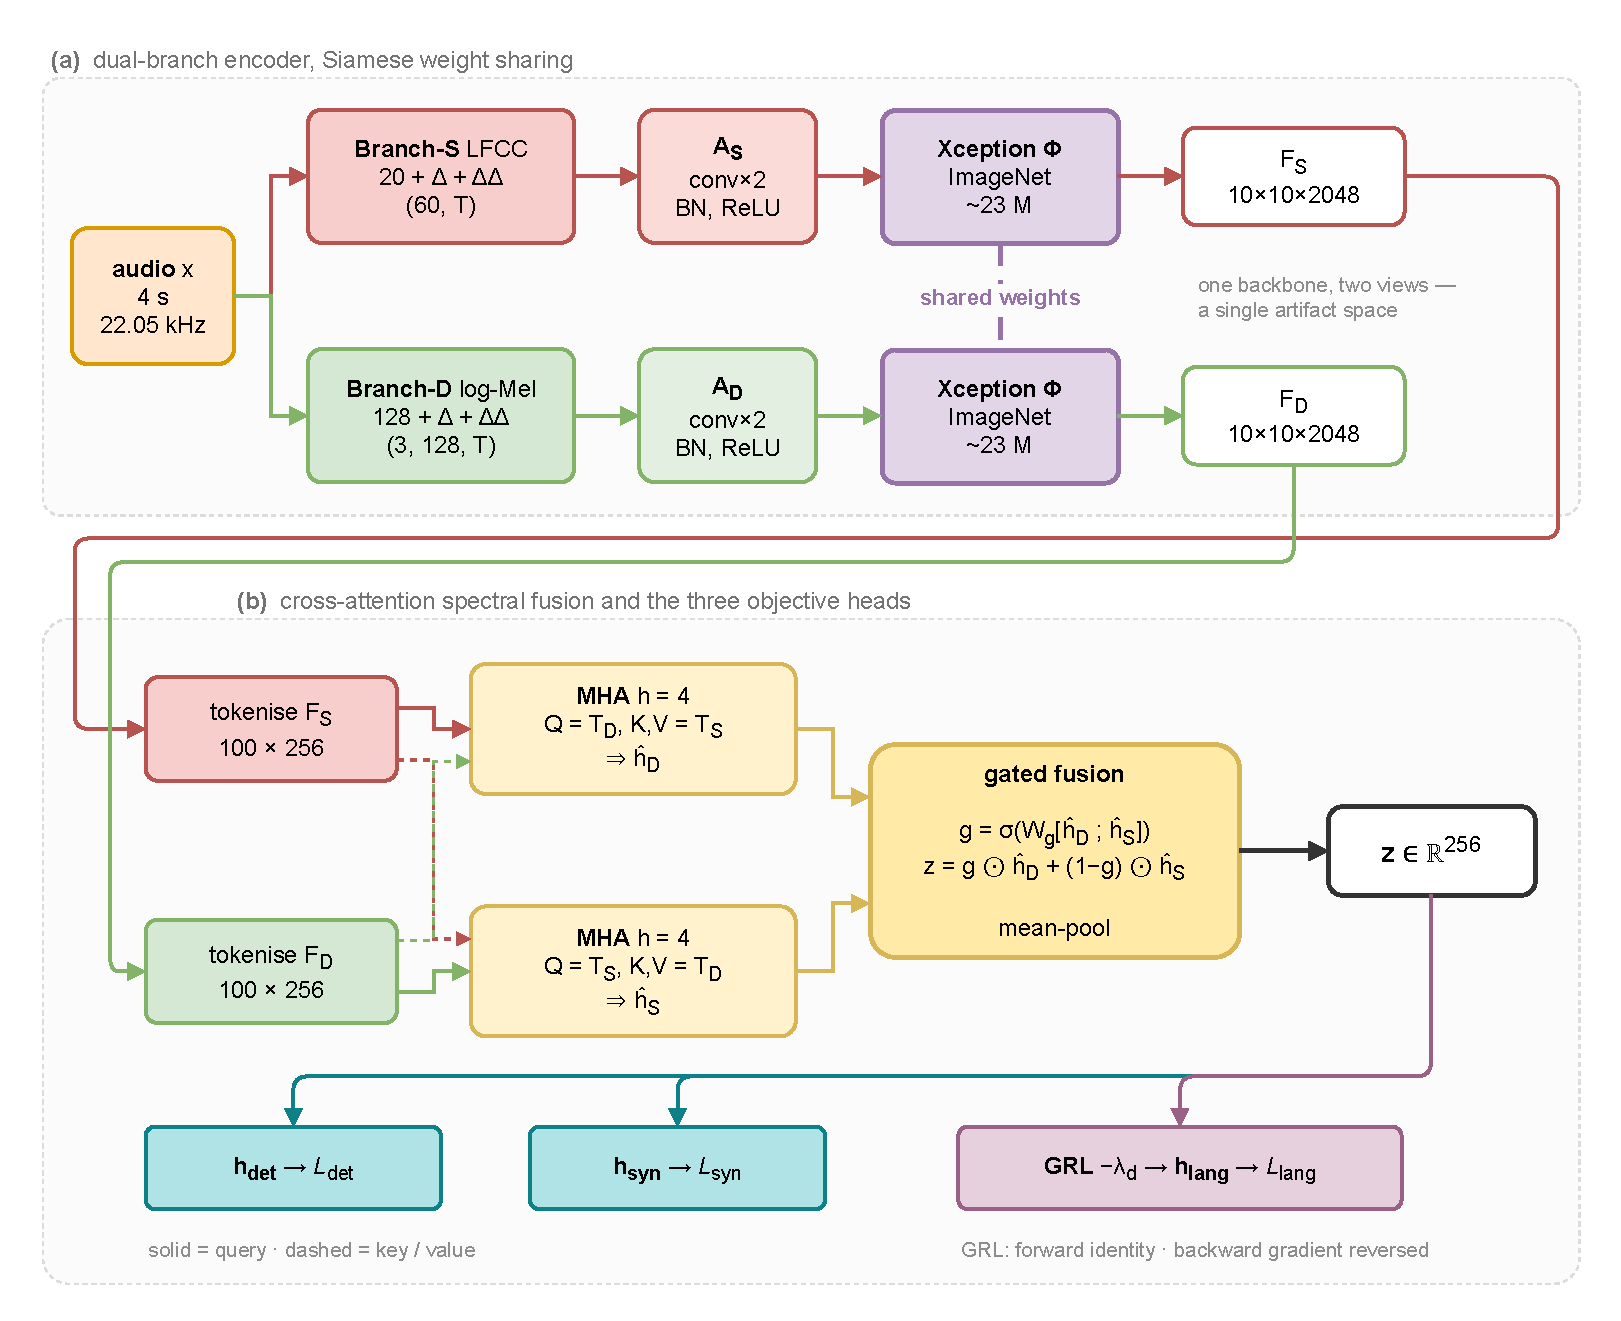
\includegraphics[width=0.96\textwidth]{fig2-dasfnet.drawio.pdf}
\caption{DASF-Net. (a) The dual-branch encoder: one utterance becomes a
sparse cepstral and a dense spectral view, each passed through its own
adapter stem into a single weight-shared Xception trunk. (b) CASF tokenises
both feature maps, lets each view attend over the other, and combines them
through a learned gate into $z$; three heads then act on $z$, the language
head behind a gradient reversal layer.}
\label{fig:dasfnet}
\end{figure*}

Each feature map is flattened into 100 spatial tokens and linearly
projected to $d = 256$, giving $T_S, T_D \in \mathbb{R}^{100 \times 256}$.
Two multi-head cross-attention blocks ($h = 4$) let each view interrogate
the other,
\begin{align}
\hat{h}_D &= \mathrm{LN}\!\left(T_D + \mathrm{MHA}(Q{=}T_D,\, K{=}T_S,\, V{=}T_S)\right),\\
\hat{h}_S &= \mathrm{LN}\!\left(T_S + \mathrm{MHA}(Q{=}T_S,\, K{=}T_D,\, V{=}T_D)\right),
\end{align}
and a learned gate mixes them elementwise before mean-pooling over tokens:
\begin{align}
g &= \sigma\!\left(W_g\,[\hat{h}_D \,;\, \hat{h}_S] + b_g\right),\\
z &= \mathrm{pool}\!\left(g \odot \hat{h}_D + (1 - g) \odot \hat{h}_S\right)
\;\in\; \mathbb{R}^{256}.
\end{align}

The gate is the point of the module. A fixed concatenation would assert
that both views always matter equally; the gate instead lets the network
decide, per utterance and per dimension, which representation carries the
artifact. It also makes the model interpretable in a way the earlier
feature comparison was not: the distribution of $g$ over a test set is a
direct, quantitative answer to ``does this generator leave its trace in
dense spectral structure or in sparse cepstral structure?'', and we
report it as an analysis in its own right.

\subsection{Objective heads}
Three heads read the same $z$.

\textbf{Detection head $h_{\mathrm{det}}$} ($256 \rightarrow 128
\rightarrow 2$) performs the task of record, real versus deepfake, under
cross-entropy with label smoothing $0.1$, giving $\Loss_{\mathrm{det}}$.

\textbf{Synthesis-family head $h_{\mathrm{syn}}$} ($256 \rightarrow 128
\rightarrow 3$) predicts \{real, GAN-vocoder, end-to-end TTS\}. This
auxiliary supervision is deliberately coarse: predicting the specific
generator would invite memorisation of generator identity, which is exactly
the failure that breaks cross-vocoder transfer, whereas predicting the
\emph{family} pushes $z$ to organise around mechanism. It contributes
$\Loss_{\mathrm{syn}}$ with a positive weight $\lambda_{\mathrm{syn}}$.

\textbf{Language head $h_{\mathrm{lang}}$} ($256 \rightarrow 128
\rightarrow 2$) predicts English versus Bengali, but sits behind a gradient
reversal layer (GRL) \cite{ganin2016dann}. The GRL is the identity in the
forward pass and multiplies the gradient by $-\lambda_d$ in the backward
pass. The head therefore does its best to identify the language while the
shared trunk and CASF are driven to make that identification impossible.
At convergence $z$ retains what distinguishes synthetic from genuine and
discards what distinguishes Bengali from English.

\subsection{The dual-adversarial objective}
Writing $\delta$ for an adversarial perturbation of the input features, the
complete training objective is
\begin{equation}
\label{eq:total}
\Loss_{\mathrm{total}} =
\Loss_{\mathrm{det}}(x)
+ \lambda_{\mathrm{adv}} \Loss_{\mathrm{det}}(x + \delta)
+ \lambda_{\mathrm{syn}} \Loss_{\mathrm{syn}}
- \lambda_{d} \Loss_{\mathrm{lang}} ,
\end{equation}
where the negative sign is realised by the GRL rather than by ascending the
loss directly. Equation~(\ref{eq:total}) contains two adversaries of
different kinds. The perturbation adversary is \emph{local}: it searches a
small neighbourhood of each input for a direction that flips the decision.
The domain adversary is \emph{global}: it searches the embedding for any
direction that reveals the corpus. Our hypothesis is that they are
complementary --- that a representation stripped of language identity
offers fewer spurious directions for a gradient attack to exploit, and that
a representation hardened against local perturbation is less able to rely
on the brittle, corpus-specific cues the domain adversary attacks. The
ablation in Section~\ref{sec:design} is designed to test that hypothesis
rather than assume it.

\subsection{Threat model}
\label{sec:threat}
We evaluate two white-box attacks in the normalised feature domain, where
inputs lie in $[0,1]$ after per-utterance standardisation. FGSM
\cite{goodfellow2015fgsm} takes a single step,
\begin{equation}
\delta_{\mathrm{FGSM}} = \epsilon \cdot \mathrm{sign}\!\left(\nabla_x \Loss_{\mathrm{det}}(x, y)\right),
\end{equation}
and PGD \cite{madry2018pgd} iterates $K = 10$ steps with step size
$\alpha = \epsilon / 4$, projecting onto the $\ell_\infty$ ball of radius
$\epsilon$ after each step. Critically, \emph{both attacks are swept over
the same $\epsilon$ grid}, $\epsilon \in \{0.001,\, 0.005,\, 0.010\}$. We
note this explicitly because prior work, including our own earlier study,
reports FGSM and PGD at $\epsilon$ values two
orders of magnitude apart, which makes the resulting robustness figures
non-comparable between the two attacks; results obtained under mismatched
budgets should not be read as evidence that one attack is stronger than the
other. All robustness numbers in this work are reported per $\epsilon$.

% =============================================================================
\section{Training Methodology}
\label{sec:training}
% =============================================================================

\begin{figure*}[!t]
\centering
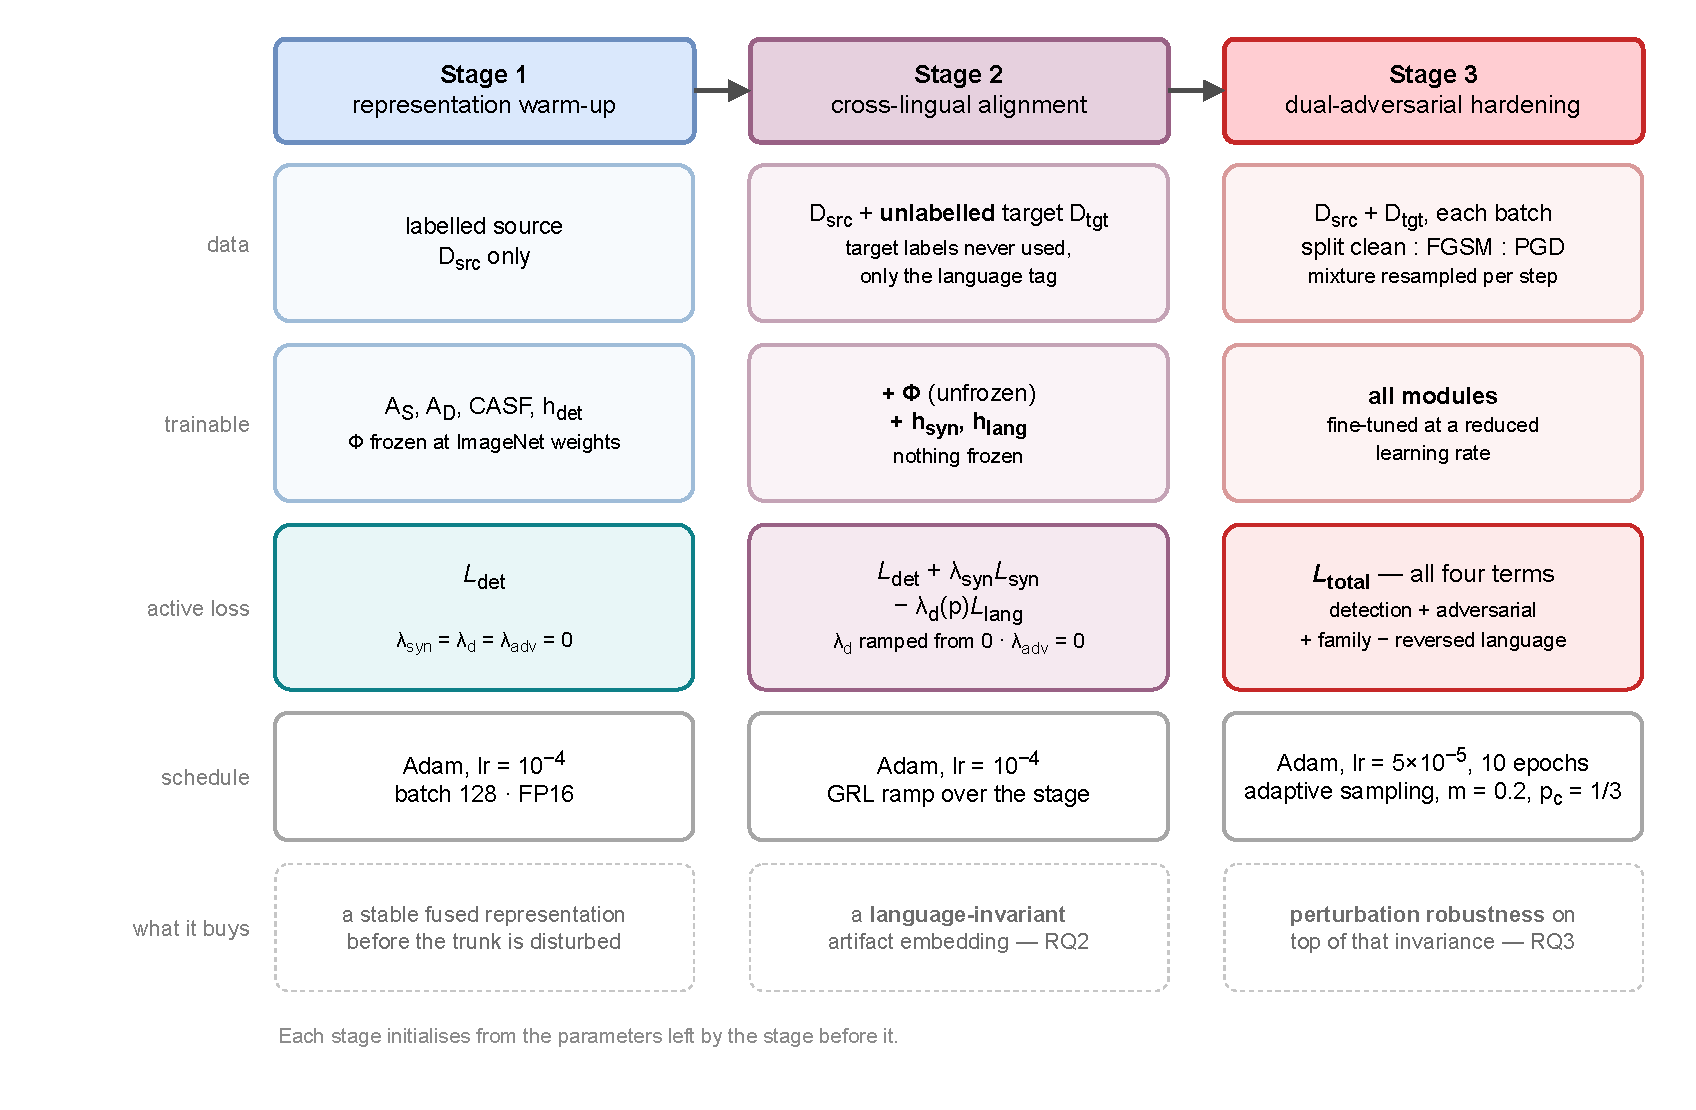
\includegraphics[width=0.94\textwidth]{fig3-training.drawio.pdf}
\caption{The three-stage curriculum. Each stage adds one source of
difficulty and inherits the weights of the stage before it: representation
warm-up over labelled source data with the trunk frozen; cross-lingual
alignment, which unfreezes the trunk and introduces the gradient-reversed
language discriminator over unlabelled target audio; and dual-adversarial
hardening, which adds adaptive FGSM/PGD sampling on top of the aligned
representation.}
\label{fig:training}
\end{figure*}

\subsection{Why a curriculum}
Training Eq.~(\ref{eq:total}) from random initialisation is unstable in
practice: a gradient-reversed discriminator applied to an untrained encoder
produces a large, uninformative reversed gradient, and adversarial examples
generated against an untrained decision boundary are meaningless. We
therefore introduce difficulty in three stages, illustrated in
Fig.~\ref{fig:training}, each initialised from the previous.

\textbf{Stage 1 --- representation warm-up.} $\Phi$ is frozen at its
ImageNet weights; only $A_S$, $A_D$, CASF and $h_{\mathrm{det}}$ train, on
labelled source data, under $\Loss_{\mathrm{det}}$ alone
($\lambda_{\mathrm{syn}} = \lambda_d = \lambda_{\mathrm{adv}} = 0$). Adam,
$lr = 10^{-4}$, batch 128, mixed precision. This establishes a usable fused
representation before the pretrained trunk is disturbed.

\textbf{Stage 2 --- cross-lingual alignment.} $\Phi$ unfreezes;
$h_{\mathrm{syn}}$ and $h_{\mathrm{lang}}$ are attached. Batches mix
labelled source audio with \emph{unlabelled} target audio: target labels
are never used, only the language tag, which keeps the setting honestly
unsupervised with respect to the target domain. Following
\cite{ganin2016dann} the reversal coefficient is ramped rather than fixed,
\begin{equation}
\lambda_d(p) = \lambda_{\max}\left(\frac{2}{1 + e^{-10p}} - 1\right),
\end{equation}
with $p \in [0,1]$ the fraction of the stage completed, so the
discriminator gains influence only as it becomes informative.

\textbf{Stage 3 --- dual-adversarial hardening.} All modules fine-tune at
$lr = 5 \times 10^{-5}$ for 10 epochs with adversarial examples introduced
by the adaptive sampler of Algorithm~\ref{alg:train}, with the language
adversary still active. Attaching robustness after alignment, rather than
before, means the perturbation adversary hardens a representation that is
already language-invariant.

\subsection{Adaptive attack sampling}
Rather than fixing the ratio of FGSM to PGD batches, we sample the attack
for each minibatch in proportion to a momentum-smoothed estimate of how
successful each attack has recently been \cite{ahmed2026melspec}. Writing
$s_a$ for the running success estimate of attack $a$ and $\hat{s}_a$ for
its measured success on the current batch,
\begin{equation}
s_a \leftarrow (1 - m)\, s_a + m\, \hat{s}_a, \qquad m = 0.2 ,
\end{equation}
and attacks are drawn with probability proportional to $s_a$ over the
non-clean fraction, while a fixed fraction $p_c = 1/3$ of every minibatch
stays clean to preserve baseline accuracy. Training therefore concentrates
on whichever attack currently works, without a hand-tuned schedule.

\subsection{Algorithms}

Algorithm~\ref{alg:forward} states the forward computation;
Algorithm~\ref{alg:train} states the training procedure.

\begin{algorithm}[t]
\caption{DASF-Net forward pass}
\label{alg:forward}
\begin{algorithmic}[1]
\REQUIRE waveform $w$; adapters $A_S, A_D$; shared trunk $\Phi$;
projection $W_p$; attention blocks; gate $W_g$; heads
$h_{\mathrm{det}}, h_{\mathrm{syn}}, h_{\mathrm{lang}}$; GRL coefficient
$\lambda_d$
\ENSURE detection logits $\hat{y}$, family logits $\hat{f}$, language
logits $\hat{\ell}$, gate $g$
\STATE $w \leftarrow$ \textsc{HBP}$(w)$ \COMMENT{22.05 kHz, trim, 4 s}
\STATE $S \leftarrow \mathrm{STFT}(w;\, n_{\mathrm{fft}}{=}2048,\, \mathrm{hop}{=}512)$
\STATE $x_S \leftarrow \mathrm{resize}\big(\Delta\Delta(\mathrm{DCT}(\mathrm{LinFB}_{20}(S)))\big)$
\STATE $x_D \leftarrow \mathrm{resize}\big(\Delta\Delta(\log \mathrm{MelFB}_{128}(S))\big)$
\STATE $F_S \leftarrow \Phi(A_S(x_S))$;\quad $F_D \leftarrow \Phi(A_D(x_D))$
\COMMENT{tied weights}
\STATE $T_S \leftarrow W_p\,\mathrm{tokens}(F_S)$;\quad $T_D \leftarrow W_p\,\mathrm{tokens}(F_D)$
\STATE $\hat{h}_D \leftarrow \mathrm{LN}(T_D + \mathrm{MHA}(T_D, T_S, T_S))$
\STATE $\hat{h}_S \leftarrow \mathrm{LN}(T_S + \mathrm{MHA}(T_S, T_D, T_D))$
\STATE $g \leftarrow \sigma(W_g [\hat{h}_D ; \hat{h}_S] + b_g)$
\STATE $z \leftarrow \mathrm{pool}\big(g \odot \hat{h}_D + (1-g) \odot \hat{h}_S\big)$
\STATE $\hat{y} \leftarrow h_{\mathrm{det}}(z)$;\quad
       $\hat{f} \leftarrow h_{\mathrm{syn}}(z)$
\STATE $\hat{\ell} \leftarrow h_{\mathrm{lang}}(\mathrm{GRL}_{\lambda_d}(z))$
\COMMENT{identity forward, $-\lambda_d$ backward}
\RETURN $\hat{y}, \hat{f}, \hat{\ell}, g$
\end{algorithmic}
\end{algorithm}

\begin{algorithm}[t]
\caption{Three-stage dual-adversarial training}
\label{alg:train}
\begin{algorithmic}[1]
\REQUIRE labelled source $\Dsrc$; unlabelled target $\Dtgt$; epoch budgets
$E_1, E_2, E_3$; weights $\lambda_{\mathrm{syn}}, \lambda_{\max},
\lambda_{\mathrm{adv}}$; momentum $m$; clean fraction $p_c$; budget grid
$\mathcal{E}$
\ENSURE trained parameters $\theta = \{A_S, A_D, \Phi, \mathrm{CASF}, h_\ast\}$
\STATE freeze $\Phi$;\quad $s_{\mathrm{FGSM}} \leftarrow s_{\mathrm{PGD}} \leftarrow 0.5$
\FOR{$e = 1$ \TO $E_1$}
  \FORALL{minibatch $B \sim \Dsrc$}
    \STATE update $\{A_S, A_D, \mathrm{CASF}, h_{\mathrm{det}}\}$ on
    $\Loss_{\mathrm{det}}(B)$
  \ENDFOR
\ENDFOR
\STATE unfreeze $\Phi$;\quad attach $h_{\mathrm{syn}}, h_{\mathrm{lang}}$
\FOR{$e = 1$ \TO $E_2$}
  \FORALL{minibatch $B = B_{\mathrm{src}} \cup B_{\mathrm{tgt}}$,
          $B_{\mathrm{src}} \sim \Dsrc$, $B_{\mathrm{tgt}} \sim \Dtgt$}
    \STATE $p \leftarrow$ fraction of Stage 2 completed
    \STATE $\lambda_d \leftarrow \lambda_{\max}\big(2/(1 + e^{-10p}) - 1\big)$
    \STATE update $\theta$ on
    $\Loss_{\mathrm{det}} + \lambda_{\mathrm{syn}}\Loss_{\mathrm{syn}}
     - \lambda_d \Loss_{\mathrm{lang}}$
    \COMMENT{$\Loss_{\mathrm{det}}, \Loss_{\mathrm{syn}}$ on
    $B_{\mathrm{src}}$ only}
  \ENDFOR
\ENDFOR
\FOR{$e = 1$ \TO $E_3$}
  \FORALL{minibatch $B$}
    \STATE split $B$ into $B_{\mathrm{clean}}$ ($p_c$) and
    $B_{\mathrm{atk}}$ ($1 - p_c$)
    \STATE $a \sim \mathrm{Categorical}\!\left(
      s_{\mathrm{FGSM}},\, s_{\mathrm{PGD}}\right)$ normalised
    \STATE $\epsilon \sim \mathrm{Uniform}(\mathcal{E})$
    \STATE $\delta \leftarrow \textsc{Attack}_a(B_{\mathrm{atk}},
    \epsilon, \theta)$
    \STATE $\hat{s}_a \leftarrow$ misclassification rate of
    $B_{\mathrm{atk}} + \delta$
    \STATE $s_a \leftarrow (1-m)\, s_a + m\, \hat{s}_a$
    \STATE update $\theta$ on Eq.~(\ref{eq:total}) over
    $B_{\mathrm{clean}} \cup (B_{\mathrm{atk}} + \delta)$
  \ENDFOR
\ENDFOR
\RETURN $\theta$
\end{algorithmic}
\end{algorithm}

\subsection{Complexity}
DASF-Net adds $0.12$~M adapter parameters, a $2048 \times 256$ projection,
two four-head attention blocks over 100 tokens, and three small MLP heads
--- together under $2$~M parameters on top of the $23$~M Xception trunk.
Because $\Phi$ is shared, the dominant training cost is that the trunk runs
twice per utterance, roughly doubling the forward and backward cost of the
single-branch baseline; Stage 3 adds the usual adversarial-training
overhead, with PGD at $K = 10$ dominating. Inference cost is two trunk
passes plus attention over 100 tokens, which remains real-time on a single
modern GPU.

% =============================================================================
\section{Experimental Design}
\label{sec:design}
% =============================================================================

This section specifies the study to be run. No results are reported.

\subsection{Research questions}
\begin{itemize}
\item \textbf{RQ1 (representation).} Does the dense-over-sparse advantage
observed for CNNs on English GAN-vocoder audio hold on Bengali VITS audio,
and does learned fusion beat either view alone?
\item \textbf{RQ2 (cross-lingual transfer).} How far does the
dual-adversarial objective close the zero-shot gap between English and
Bengali, in both directions, relative to a non-adversarial baseline?
\item \textbf{RQ3 (robustness transfer).} Does adversarial robustness
acquired on one language survive transfer to the other, and does language
invariance make that transfer easier?
\end{itemize}

\subsection{Confound-Controlled Evaluation Protocol}
\label{sec:ccep}
Every figure reported under this protocol is subject to four constraints,
which follow directly from the confounds of Section~\ref{sec:pairing}.

\begin{enumerate}
\item \textbf{Speaker-disjoint splits.} No speaker appears in both training
and test partitions, so a model cannot succeed by speaker recognition.
\item \textbf{Gender-balanced Bengali evaluation.} Because BanglaFake pairs
one male synthetic speaker against mixed-gender real speech, the primary
Bengali test set is restricted to male real speech, and the mixed-gender
result is reported separately as a diagnostic. A large gap between the two
is itself evidence of gender shortcutting.
\item \textbf{Prior-matched test sets.} Both test sets are resampled to
$1{:}1$ real-to-synthetic, so that accuracy is interpretable and comparable
across domains.
\item \textbf{Threshold-free primary metric.} EER is the headline metric,
with min-tDCF \cite{kinnunen2018tdcf} and balanced accuracy alongside it.
Raw accuracy is never reported for a transfer condition without its
matching prior.
\end{enumerate}

\subsection{Experiments}
\textbf{E1 --- In-language baselines.} Train and evaluate on each corpus
separately: Branch-S only, Branch-D only, and full CASF fusion. Compare
against the published ResNet18 fine-tuned baseline
(79.17\% accuracy, 0.2435 EER) and the single-branch Xception of our prior
study. Addresses RQ1 and calibrates everything that follows.

\textbf{E2 --- Zero-shot transfer.} Train on the source and evaluate on the
target without target labels, in both directions: EN$\rightarrow$BN, and
BN$\rightarrow$EN with a per-vocoder breakdown over the seven WaveFake
generators. Each direction is run with and without the language adversary,
which isolates the contribution of Stage 2. A few-shot variant fine-tunes
on $\leq 10\%$ of target data to characterise how quickly the gap closes
with minimal supervision. Addresses RQ2.

\textbf{E3 --- Robustness and its transfer.} Under the threat model of
Section~\ref{sec:threat}, report clean, FGSM and PGD EER per $\epsilon$ for
(i) a model adversarially trained and tested in-domain, and (ii) a model
adversarially trained on the source and tested on the target. The gap
between them measures how language-specific robustness is. Addresses RQ3.

\textbf{E4 --- Ablation.} Removing one component at a time from the full
model: no CASF (concatenation instead of gated cross-attention); no shared
trunk (independent backbones); no $h_{\mathrm{syn}}$; no GRL; no
adversarial stage; and 16~kHz preprocessing in place of HBP. This is what
converts an observed improvement into an attributed one, and the 16~kHz row
in particular tests whether the bandwidth argument of
Section~\ref{sec:hbp} holds empirically.

\textbf{E5 --- Gate analysis.} Report the distribution of the fusion gate
$g$ per generator family. This asks directly whether GAN vocoders and
end-to-end TTS leave their traces in different representations, and gives
the fusion module an interpretable output rather than only an accuracy
delta.

\subsection{Implementation}
PyTorch with mixed-precision training, Adam throughout, batch size 128,
label smoothing $0.1$. Adversarial attacks are implemented in the
normalised feature domain described in Section~\ref{sec:threat}. Every
experiment is run with three random seeds and reported as mean and standard
deviation; single-seed results are not reported. Code, split definitions
and evaluation scripts will be released with the empirical paper.

% =============================================================================
\section{Limitations and Threats to Validity}
% =============================================================================

We state these in advance because several bound what the planned study can
conclude, regardless of its outcome.

\textbf{One Bengali generator.} BanglaFake contains a single VITS system,
so this design tests cross-\emph{paradigm} generalisation but cannot test
cross-vocoder generalisation \emph{within} Bengali the way WaveFake's
seven-generator leave-one-out protocol does for English. A claim that
DASF-Net generalises across Bengali synthesisers would not be supported by
this data, and we do not intend to make one. Extending BanglaFake with a
Bengali FastSpeech2 or Tacotron2 system is the natural next step.

\textbf{Confounds mitigated, not eliminated.} CCEP controls speaker,
gender and prior, but each control shrinks the usable Bengali evaluation
set, trading statistical power for validity. Both the controlled and
uncontrolled figures should be read together.

\textbf{White-box attacks only.} FGSM and PGD assume full gradient access.
Black-box, transfer, perceptual and physical-channel attacks are outside
this design, and robustness claims should be read as bounded by that.

\textbf{Two languages.} Bengali and English differ in phoneme inventory,
prosody and recording conditions simultaneously. Language invariance
demonstrated over one pair is evidence, not proof, of invariance in
general.

\textbf{Adversarial cost.} Stage 3 roughly doubles training time on top of
the doubled forward cost of the two-branch encoder, which matters for
reproduction on modest hardware.

% =============================================================================
\section{Conclusion}
% =============================================================================

We have presented DASF-Net, an architecture that treats the two standing
weaknesses of audio deepfake detectors --- brittleness across languages and
brittleness under perturbation --- as instances of the same problem, and
attacks both with adversaries acting on one shared embedding. The
architecture contributes a dual-branch spectral front-end over a
Siamese-shared Xception trunk, a gated cross-attention fusion module that
learns per utterance which spectral view carries the artifact, and a
combined objective in which a gradient-reversed language discriminator and
adaptive FGSM/PGD training shape the same representation. We have specified
the three-stage curriculum that makes this trainable, the algorithms in
full, a corrected and unit-consistent adversarial threat model, and a
Confound-Controlled Evaluation Protocol that neutralises the speaker,
gender and prior imbalances which otherwise make Bengali detection results
unreadable.

What the design buys, if the hypothesis holds, is a detector whose features
describe what a synthesiser did rather than which corpus it was trained on.
Whether it does hold is an empirical question, and the experiments of
Section~\ref{sec:design} --- in particular the ablation that separates the
fusion module from the language adversary from the perturbation adversary
--- are constructed to answer it in a way that attributes any gain to a
specific cause. Those results are reported separately.

% =============================================================================
\iffalse
\begin{thebibliography}{00}

\bibitem{kong2020hifigan}
J.~Kong, J.~Kim, and J.~Bae, ``HiFi-GAN: Generative adversarial networks
for efficient and high fidelity speech synthesis,'' in \emph{Advances in
Neural Information Processing Systems (NeurIPS)}, vol.~33, 2020,
pp.~17022--17033.

\bibitem{kumar2019melgan}
K.~Kumar, R.~Kumar, T.~de~Boissiere, L.~Gestin, W.~Z.~Teoh, J.~Sotelo,
A.~de~Br\'{e}bisson, Y.~Bengio, and A.~Courville, ``MelGAN: Generative
adversarial networks for conditional waveform synthesis,'' in
\emph{Advances in Neural Information Processing Systems (NeurIPS)},
vol.~32, 2019, pp.~14910--14921.

\bibitem{prenger2019waveglow}
R.~J.~Prenger, R.~Valle, and B.~Catanzaro, ``WaveGlow: A flow-based
generative network for speech synthesis,'' in \emph{Proc.\ ICASSP}, 2019,
pp.~3617--3621.

\bibitem{yamamoto2020pwg}
R.~Yamamoto, E.~Song, and J.-M.~Kim, ``Parallel WaveGAN: A fast waveform
generation model based on generative adversarial networks with
multi-resolution spectrogram,'' in \emph{Proc.\ ICASSP}, 2020,
pp.~6199--6203.

\bibitem{kim2021vits}
J.~Kim, J.~Kong, and J.~Son, ``Conditional variational autoencoder with
adversarial learning for end-to-end text-to-speech,'' in \emph{Proc.\
International Conference on Machine Learning (ICML)}, 2021, pp.~5530--5540.

\bibitem{todisco2019asvspoof}
M.~Todisco, X.~Wang, V.~Vestman, M.~Sahidullah, H.~Delgado, A.~Nautsch,
J.~Yamagishi, N.~Evans, T.~H.~Kinnunen, and K.~A.~Lee, ``ASVspoof 2019:
Future horizons in spoofed and fake audio detection,'' in \emph{Proc.\
Interspeech}, 2019, pp.~1008--1012.

\bibitem{frank2021wavefake}
J.~Frank and L.~Sch\"{o}nherr, ``WaveFake: A data set to facilitate audio
deepfake detection,'' in \emph{35th Conference on Neural Information
Processing Systems (NeurIPS) Datasets and Benchmarks Track}, 2021.

\bibitem{fahad2025banglafake}
I.~A.~Fahad, K.~Asif, and S.~Sikder, ``BanglaFake: Constructing and
evaluating a specialized Bengali deepfake audio dataset,''
\emph{arXiv preprint arXiv:2505.10885}, 2025.

\bibitem{samu2025zeroshot}
M.~S.~S.~Samu, M.~R.~Islam, M.~Z.~Hossain, M.~K.~Bhuiyan, and
F.~U.~Zaman, ``Zero-shot to zero-lies: Detecting Bengali deepfake audio
through transfer learning,'' in \emph{2025 28th International Conference
on Computer and Information Technology (ICCIT)}, 2025.

\bibitem{ahmed2026melspec}
I.~Ahmed, M.~I.~Arian, and N.~J.~Lisa, ``Mel-Spectrogram representations
for CNN based adversarial defense for audio deepfake detection,''
in \emph{Proc.\ 2026 11th International Conference on Machine Learning
Technologies (ICMLT)}, Berlin, Germany, 2026.

\bibitem{chollet2017xception}
F.~Chollet, ``Xception: Deep learning with depthwise separable
convolutions,'' in \emph{Proc.\ IEEE Conf.\ on Computer Vision and
Pattern Recognition (CVPR)}, 2017, pp.~1800--1807.

\bibitem{ganin2016dann}
Y.~Ganin, E.~Ustinova, H.~Ajakan, P.~Germain, H.~Larochelle,
F.~Laviolette, M.~Marchand, and V.~Lempitsky, ``Domain-adversarial training
of neural networks,'' \emph{Journal of Machine Learning Research}, vol.~17,
no.~59, pp.~1--35, 2016.

\bibitem{vaswani2017attention}
A.~Vaswani, N.~Shazeer, N.~Parmar, J.~Uszkoreit, L.~Jones, A.~N.~Gomez,
{\L}.~Kaiser, and I.~Polosukhin, ``Attention is all you need,'' in
\emph{Advances in Neural Information Processing Systems (NeurIPS)},
vol.~30, 2017, pp.~5998--6008.

\bibitem{goodfellow2015fgsm}
I.~J.~Goodfellow, J.~Shlens, and C.~Szegedy, ``Explaining and harnessing
adversarial examples,'' in \emph{Proc.\ ICLR}, 2015.

\bibitem{madry2018pgd}
A.~Madry, A.~Makelov, L.~Schmidt, D.~Tsipras, and A.~Vladu, ``Towards
deep learning models resistant to adversarial attacks,'' in \emph{Proc.\
ICLR}, 2018.

\bibitem{kawa2023lcnn}
P.~Kawa, M.~Plata, and P.~Syga, ``Defense against adversarial attacks on
audio deepfake detection,'' in \emph{Proc.\ Interspeech}, 2023,
pp.~5276--5280.

\bibitem{kinnunen2018tdcf}
T.~Kinnunen, K.~A.~Lee, H.~Delgado, N.~Evans, M.~Todisco, M.~Sahidullah,
J.~Yamagishi, and D.~A.~Reynolds, ``t-DCF: A detection cost function for
the tandem assessment of spoofing countermeasures and automatic speaker
verification,'' in \emph{Proc.\ Odyssey}, 2018, pp.~312--319.

\bibitem{ito2017ljspeech}
K.~Ito and L.~Johnson, ``The LJ speech dataset,''
\url{https://keithito.com/LJ-Speech-Dataset/}, 2017.

\bibitem{ahmad2021sust}
A.~Ahmad, M.~Selim, M.~Iqbal, and M.~Rahman, ``SUST TTS corpus: A
phonetically balanced corpus for Bangla text-to-speech synthesis,''
\emph{Acoustical Science and Technology}, vol.~42, no.~6, pp.~326--332,
2021.

\bibitem{ardila2020commonvoice}
R.~Ardila, M.~Branson, K.~Davis, M.~Henretty, M.~Kohler, J.~Meyer,
R.~Morais, L.~Saunders, F.~M.~Tyers, and G.~Weber, ``Common Voice: A
massively-multilingual speech corpus,'' in \emph{Proc.\ 12th Conference on
Language Resources and Evaluation (LREC)}, 2020, pp.~4211--4215.

\end{thebibliography}
\fi

\end{document}
